\subsection{SMS decomposition: The procedure}
\label{ssec:decomp}


As discussed in Sec.\ref{ssec:names}, within the SMS philosophy all the information
about the BSM model is encapsulated in the production cross-sections of the new
($\mathbb{Z}_2$-odd) states, their masses and branching ratios.
The latter two can be easily specified by a SLHA file, containing the
mass spectrum and decay table of the model.
However, to obtain the production cross-sections it is necessary to use
additional tools, which evaluate $\sigma$ for the specific BSM model of interest.
Since we will present results for the MSSM, we use Pythia\cite{pythia} and NLL-fast\cite{NLLfast} to 
generate the cross-sections for sparticle pair production.


In order to translate the BSM information contained in the SLHA input file and production
cross-sections to the SMS topologies, we apply our decomposition procedure, which
begins with the pair production cross-sections. Starting with the two mother particles
produced in the hard scattering, we use the SLHA decay table to produce all possible distinct cascade decays of the 
mother particles\footnote{In practice we remove all cascade decays with $\sigmaXBF$ below a certain threshold
to eliminate irrelevant topologies.}. Repeating this procedure for each pair of mothers with non-negligible
production cross-sections we obtain all relevant SMS topologies.
The weight ($\sigmaXBF$) of each topology can then be computed as the mother's production cross-section times
all the branching ratios appearing in the SMS topology.
Finally, for each topology, a list of masses for the BSM states appearing in it is also obtained
from the SLHA spectrum. Therefore, from the production cross-sections and the SLHA input file,
we produce all possible topologies as well as obtain all the information concerning each
single topology: number of vertices, SM final states in each vertex, masses of BSM states and weight.
Note that if two identical topologies ($[B_1,B_2] = [B_1',B_2']$) appearing from two distinct cascade
decays, have identical mass lists, their weights will be automatically added, since in our framework they are indistinguisable.
With the decomposition procedure just described all the theoretical uncertainty is restricted to the
uncertainties in the cross-section calculation (assuming neglegible errors for the mass spectrum
and branching ratios). Finally, we point out that the decompostion can also be made using an LHE
event file, where parton level events are stored containing all relevant production and cascade decays.
Although this method is more flexible, since it does not require an SLHA input file,
it is also more prone to Monte Carlo (MC) uncertainties and we do not adopt it for our subsequent
results.


Using the procedure described above it is possible to decompose a BSM model into
a series of SMS topologies with their respective weights. All the relevant information
for confronting the model with the experimental results is then encapsulated in the SMS
topologies (plus their masses and weights) and any specific model dependent information (such as the
SLHA input file and the calculation of model specific cross-sections) can be dropped at this point.
Before a direct comparison with the experimental constraints, two more steps are required.
The first step consists in combining single topologies (which means adding their weights)
according to the experimental analysis' assumptions. As discussed in Sec.\ref{ssec:smsstatistics}, 
it is often the case that the experimental collaboration chooses to constrain
a sum of SMS topologies instead of a single one.
In most cases the sum is trivial and consists in adding topologies which only differ by the
lepton flavor in the final state (as exemplified in Sec.\ref{ssec:smsstatistics}) and/or final state charges.
In other cases the sum is over distinct final state particles. Nonetheless, in all cases only topologies with the same
overall shape (number of vertices and number of SM particles in each vertex) are added together. 
Also, the sum must be restricted to topologies
with identical masses, otherwise signal topologies with very distinct kinematics would be
combined. 

The final step for computing the relevant theoretical cross-sections consists of identifying quasi-degenerate masses appearing in the BSM spectrum.
It is often the case that two BSM particles have similar masses and, for all experimental purposes, 
can be considered to be degenerate. Standard examples are the $\tilde{e}$ and $\tilde{\mu}$ masses
or the $\chipm$ and $\chitz$ masses in some regions of the MSSM parameter space.
Identifying similar masses is essential to evaluate the theoretical prediction
for a specific analysis, since only topologies with identical (or similar) masses can be combined, as discussed above.
Since different experimental analyses may have distinct sensitivities to mass splittings,
we introduce an analysis-dependent "mass distance", which measures how much the experimental 
upper limit changes from one mass value to the other.
If the two masses are very close together (there is no significant change in the UL),
we consider the two masses equal for this particular analysis and replace them by their average.
Then it is possible to reduce the number of unknown masses in a single topology, as in the case
of $\chipm$-$\chitz$ production with $m_{\chipm} \sim m_{\chitz}$. It also makes it possible to combine (when needed) distinct topologies
with similar mass lists, as in the case of $\tilde{e}^+\tilde{e}^- + \tilde{\mu}^+\tilde{\mu}^-$ discussed in Sec.\ref{ssec:smsstatistics}
with $m_{\tilde{e}} \sim m_{\tilde{\mu}}$.


Once all the above steps have been performed we can directly compare the theoretical weights (\sigmaXBF) obtained for a SMS
topology (or sum of topologies) to the experimental upper limit for the respective topology and mass list value.
In Fig.\ref{fig:smsdecomposition} we sketch the main steps required to confront the BSM model predictions with the 
experimental constraints. The three main steps shown are: the SMS decomposition (based on the SLHA input file and the cross-section calculator),
the combination of SMS topologies with identical or similar masses into the topology sums assumed by the analyses and finally the
comparison with the experimental upper limits obtained from the database of LHC results described in Sec.\ref{ssec:lhc}.


\begin{figure}[h!t]\centering
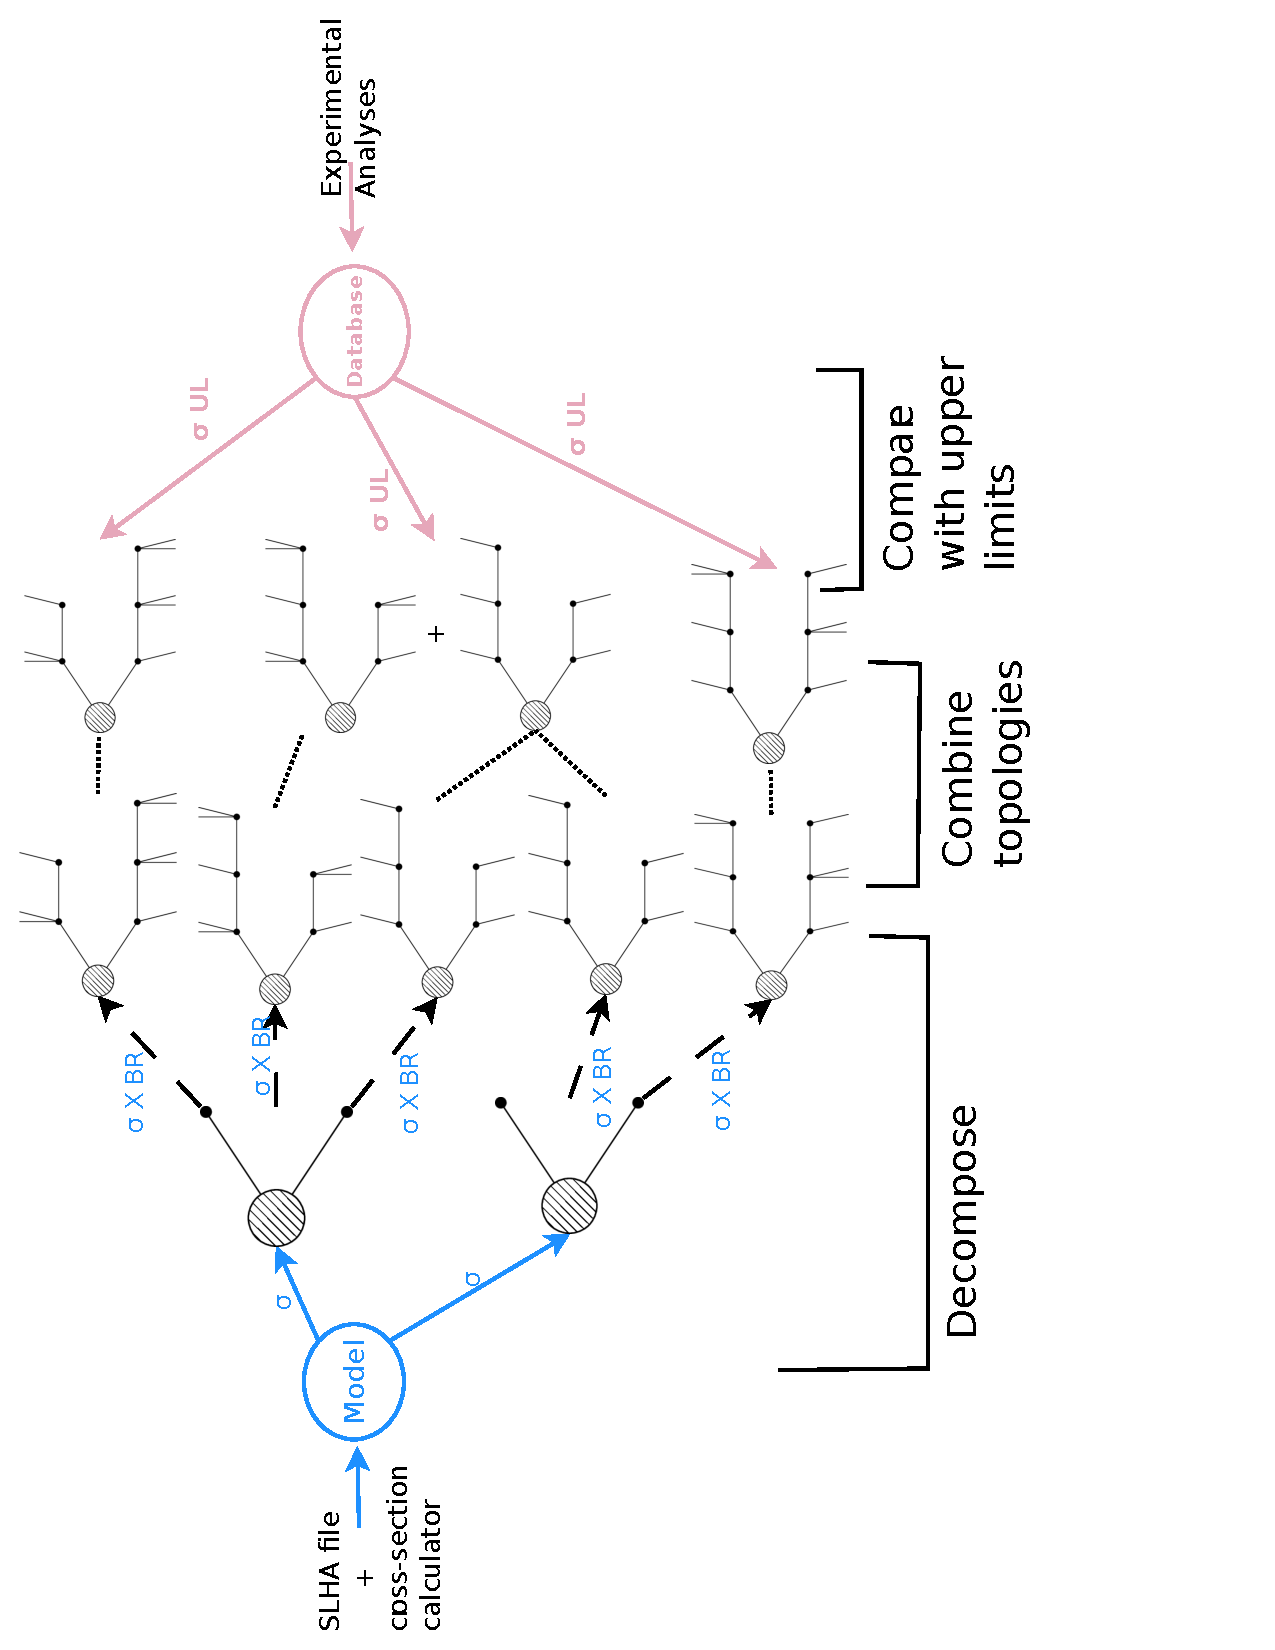
\includegraphics[width=0.9\linewidth,clip,angle=270]{figures/Scheme1.pdf}
\label{fig:smsdecomposition}
\caption{Schematics of the whole SMS decomposition procedure \fixme{Just a rough idea. Any changes are welcome}.}
\end{figure}


\FloatBarrier
